\documentclass[portrait,final,x11names,a1paper,fontscale=0.4]{baposter}

\usepackage{calc}
\usepackage{graphicx,caption}
\usepackage{relsize}
\usepackage{multirow}
\usepackage{rotating}
\usepackage{bm}
\usepackage{url}

\usepackage{graphicx,subfigure}
\usepackage{multicol}

\usepackage{microtype}
\usepackage{helvet}
\renewcommand{\familydefault}{\sfdefault}
\renewcommand{\ttdefault}{lmtt}

% Mathematics
\usepackage{amsmath,amsfonts,amsthm,amssymb,bm}
\usepackage{dutchcal}

\usepackage{numprint}
\npthousandsep{,}\npthousandthpartsep{}\npdecimalsign{.}	

\usepackage{mathtools}
\mathtoolsset{showonlyrefs}

% Valore atteso
\newcommand{\E}[1]{\mathbb{E}(#1)}

% Valore atteso condizionato
\newcommand{\Econd}[2]{\mathbb{E}(#1 \vert #2)}

% Varianza
\DeclareMathOperator{\var}{Var}

% Covarianza
\DeclareMathOperator{\cov}{Cov}

% Correlazione
\newcommand{\corr}[2]{\mathrm{Cor}(#1,#2)}

% Valore assoluto
\newcommand{\abs}[1]{\vert #1 \vert}

% Derivate
\newcommand{\der}[1]{\frac{\partial}{\partial #1}}
\newcommand{\dder}[1]{\frac{\partial^2}{\partial #1^2}}

% Spazio elenchi
\newcommand{\spazio}{\vspace{1.5em}}
\newcommand{\sspazio}{\vspace{3em}}

% Vettore bold
\renewcommand{\vec}[1]{\mathbf{#1}}

\newcommand{\field}[1]{\mathbb{#1}}
\newcommand{\olsbeta}{\hat{\bm{\beta}}_\text{OLS}}

% Math operators
%\DeclareMathOperator*{\argmax}{argmax}
\DeclareMathOperator*{\argmin}{argmin}
\DeclareMathOperator*{\plim}{plim}
\DeclareMathOperator*{\logit}{logit}
\DeclareMathOperator*{\sgn}{sgn}

\newcommand{\widesim}[2][2]{
  \mathrel{\overset{#2}{\scalebox{#1}[1]{$\sim$}}}
  }
  
% Norm
\newcommand{\norm}[1]{\left\lVert#1\right\rVert}

% Rank
\DeclareMathOperator{\rank}{rank}

% Trace
\DeclareMathOperator{\trace}{tr}

% Projection
\DeclareMathOperator*{\proj}{proj_{\perp}}

% Odds
\newcommand{\odds}{\mathrm{Odds}}

% Complementary set
\newcommand{\compl}{\mathsf{c}}

% Function floor
\newcommand{\floor}[1]{\left\lfloor #1 \right\rfloor}

% Function ceiling
\newcommand{\ceil}[1]{\left\lceil #1 \right\rceil}

% Nearest integer function
\newcommand{\nint}[1]{\left\lfloor #1 \right\rceil}

% Indicator function
\usepackage{dsfont}
\newcommand{\indfun}[2]{\mathds{1}_{#1}(#2)}

% Circled numbers
\newcommand*\circled[1]{\tikz[baseline=(char.base)]{
            \node[shape=circle,draw,inner sep=2pt] (char) {#1};}}
     
% Circled numbers (fixed radius)       
\newcommand*\circlef[1]{\tikz[baseline=(char.base)]{
  \draw[fill=white] circle [radius=0.55cm];
  \node[inner sep=2pt] (char) {#1};
}}

% Theorems, definitions, proofs
\newtheorem{theorem}{Theorem}[section]
\newtheorem{proposition}[theorem]{Proposition}
\newtheorem{corollary}{Corollary}[theorem]
\newtheorem{lemma}[theorem]{Lemma}

\newenvironment{definition}[1][Definition]{\begin{trivlist}
\item[\hskip \labelsep {\bfseries #1}]}{\end{trivlist}}

\newenvironment{example}[1][Example]{\begin{trivlist}
\item[\hskip \labelsep {\bfseries #1}]}{\end{trivlist}}

\newenvironment{remark}[1][Remark]{\begin{trivlist}
\item[\hskip \labelsep {\bfseries #1}]}{\end{trivlist}}

\newcommand{\card}[1]{\left\vert #1 \right\vert}

\DeclareMathOperator{\diri}{DP}
\DeclareMathOperator{\ibp}{IBP}
\DeclareMathOperator{\crp}{CRP}


\usepackage[font=small,labelfont=bf,textfont=it]{caption}

\setlength{\columnsep}{1.5em}
\setlength{\columnseprule}{0mm}

\usepackage{enumitem}
\setlist{noitemsep,nolistsep}
\usepackage{stackengine,fontawesome}

\usepackage{tabu}
\usepackage{multicol}
\usepackage{multirow}

\definecolor{blue_icl}{RGB}{0,62,116}
\definecolor{blue_icl2}{RGB}{0,40,255}
\definecolor{navy_icl}{RGB}{0,33,71}
\definecolor{cool_icl}{RGB}{0,110,175}

\newcommand{\icl}[1]{{\bf\color{blue_icl2}{#1}}}

\DeclareMathOperator{\argmax}{argmax}
\usepackage{bm}

\newcommand{\codepath}{./}
\usepackage{minted}
\usemintedstyle{lovelace}
\newcommand{\includeshell}[1] {\inputminted[firstline=1,fontsize=\footnotesize,breaklines]{shell-session}{\codepath/#1}}

% Vettore bold
\renewcommand{\vec}[1]{\boldsymbol{#1}}
\newcommand{\mvec}[1]{\mathbf{#1}}

\usepackage{tcolorbox}
\tcbuselibrary{theorems}
\newtcbtheorem{defi}{Definition}%
{colback=blue_icl2!5,colframe=blue_icl2,fonttitle=\bfseries,left=2pt,right=2pt,top=2pt,bottom=2pt}{th}

% Tables
\usepackage{booktabs}	
\usepackage{array,tabu}
\usepackage{multicol}
\usepackage{multirow}

\begin{document}

\begin{poster}%
  % Poster Options
  {
  % Show grid to help with alignment
  grid=false,
  % Column spacing
  colspacing=1em,
  % Color style
  bgColorOne=white,
  bgColorTwo=white,
  borderColor=blue_icl2,
  headerColorOne=cool_icl,
  headerColorTwo=blue_icl2,
  headerFontColor=white,
  boxColorOne=white,
  boxColorTwo=blue_icl2,
  % Format of textbox
  textborder=roundedleft,
  % Format of text header
  eyecatcher=true,
  headerborder=closed,
  headerheight=0.15\textheight,
  textfont=\bf,
  headershape=roundedright,
  % headershade=shadelr,
  headerfont=\Large\bf,
  textfont={\setlength{\parindent}{1.5em}},
  %boxshade=plain,
  % background=shade-tb,
  % background=plain,
  % bgColorOne=DarkOrange2!40,
  linewidth=2pt,
  columns=5
  }
  % Eye Catcher
  {\includegraphics[width=14em]{icl_eye.pdf}}%{imperial_logo.pdf}} 
  % Title
  {\centering\color{blue_icl2}{\bf{\huge Automating the selection of  preprocessing  \\[0.1cm]techniques for deep neural networks}}\vspace{0.5em}}
  % Authors
  {\vspace*{-.3cm}
  \hspace*{.8cm} 
  \leavevmode\hbox to \linewidth{ \color{blue_icl2}% 
  \centering
\begin{tabular}[t]{c@{}}
    {\Large{\textbf{Student:} Marcus September}} \\[.05cm]
    {\Large{\textbf{Supervisor:} Francesco Sanna Passino}} \\[.05cm]
\faUniversity\ {Department of Mathematics, Imperial College London} \\
\faEnvelopeO\ {\tt marcus.september22@imperial.ac.uk} \\
%{\large This work is funded by a {\bf Microsoft Security AI} research grant.}
\end{tabular} 
}}

  % University logo
%  {% The makebox allows the title to flow into the logo, this is a hack because of the L shaped logo.
    % \includegraphics[height=9.0em]{images/logo}
%  }

\headerbox{3. Exploratory data analysis}{name=ack,column=0,above=bottom,span=2}{
%\vspace*{.2cm}
 %%%%%%%%%%%%%%%%%%%%%%%%%%%%%%%%%%%%%%%%%%%%%%%%%%%%%%%%%%%%%%%%%%%%%%%%%%%%%%
%\begin{minipage}[t]{0.25\linewidth}
%\hspace*{-0.5cm}
%\includegraphics[width=0.95\textwidth]{1920px-M_box.png}
%\end{minipage} \ \hspace{-0.5cm}
%\begin{minipage}[b]{0.7\linewidth} %\smaller
\noindent
\includegraphics[width=0.48\textwidth]{Figures/eda1.png}
\includegraphics[width=0.48\textwidth]{Figures/eda2.png}
\includegraphics[width=0.48\textwidth]{Figures/eda1.png}
\includegraphics[width=0.48\textwidth]{Figures/eda2.png}

\noindent
A lot of the variables have very skewed distributions or extreme values. There are also many missing values.

%\end{minipage}
%\vspace{.25cm}
%\medskip
}

%%%%%%%%%%%%%%%%%%%%%%%%%%%%%%%%%%%%%%%%%%%%%%%%%%%%%%%%%%%%%%%%%%%%%%%%%%%%%%
  \headerbox{1. Problem and motivation}{name=problem,column=0,row=0,span=2}{
%%%%%%%%%%%%%%%%%%%%%%%%%%%%%%%%%%%%%%%%%%%%%%%%%%%%%%%%%%%%%%%%%%%%%%%%%%%%%%

\noindent   
Deep learning sequence models, such as Recurrent Neural Networks (RNNs) and
transformers, are sensitive to input variable distributions. Both training
speed and performance can drop significantly for non-normal distributions, such
as skewed distributions and those with outliers. Real-world data also usually
contains a lot of missing values, which needs to be converted to numeric values
for use in deep learning models. Deciding on appropriate preprocessing methods
and how to handle missing values is essential in optimising model performance.
However, this is a time-consuming process. The project aims to automate this by
automatically selecting the preprocessing methods to use for any given
sequence dataset, in order to optimise performance and training efficiency.
}


%%%%%%%%%%%%%%%%%%%%%%%%%%%%%%%%%%%%%%%%%%%%%%%%%%%%%%%%%%%%%%%%%%%%%%%%%%%%%%
\headerbox{2. Data}{name=data,column=0,row=1,below=problem,above=ack,span=2}{
%%%%%%%%%%%%%%%%%%%%%%%%%%%%%%%%%%%%%%%%%%%%%%%%%%%%%%%%%%%%%%%%%%%%%%%%%%%%%%
\noindent
Dataset consists of $N\approx 460000$ customers, each with $P=188$ aggregated
profile features recorded at each of the $T=13$ sequential statement dates.
Together, the dataset forms $N$ instances of a $P$-dimensional multivariate
time-series of length $T$. For each multivariate time-series, the target label
$y \in \{0,1\}$ indicates whether the customer defaulted on their loan or not.
The task is to predict the probability $\mathbb{P}(Y=1)$. Note that due to
privacy concerns, all the dataset features have been anonymized. 
TODO: say something about anonymised with random noise.
}


%%%%%%%%%%%%%%%%%%%%%%%%%%%%%%%%%%%%%%%%%%%%%%%%%%%%%%%%%%%%%%%%%%%%%%%%%%%%%%
\headerbox{4. Synthetic data}{name=meg,column=2,span=3,row=0, aligned=problem}{
%%%%%%%%%%%%%%%%%%%%%%%%%%%%%%%%%%%%%%%%%%%%%%%%%%%%%%%%%%%%%%%%%%%%%%%%%%%%%%

\noindent
\begin{itemize}[leftmargin=.15in]
\item 
With the synthetic data generation procedure I have proposed, I can specify arbitrary unnormalized probability density functions (PDFs) for each of the $P$ variables, from which the inverse cumulative
density functions, $F^{-1}_1,\dots,F^{-1}_P$ are inferred. Correlated uniform random variables
$U \in [0,1]^{T \times P}$
with a similar correlation structure as that of a multivariate time-series are then generated,
and a response $y \in \{0,1\}$ is formed from these. These uniform random variables are then
transformed by $F^{-1}_1,\dots,F^{-1}_P$ and returned to the user with the response, as samples from the provided PDFs.
% TODO: could maybe replace this with a diagram of $U$s, arrow down to $X$s, and arrow right to response. Could also shorten the explanation to just emphasize fact that I can specify the PDFs
\item  By being able to fully control the distribution of each variable, it will be easier to experiment and learn \textit{when} each preprocessing method works best, and this insight can be used to
    form the heuristics used for automatically selection the appropriate techniques.
\end{itemize}


}

%%%%%%%%%%%%%%%%%%%%%%%%%%%%%%%%%%%%%%%%%%%%%%%%%%%%%%%%%%%%%%%%%%%%%%%%%%%%%%
\headerbox{5. Preliminary result I: Preprocessing on real data}{name=picture,column=2,span=3,row=1, below=meg}{
%%%%%%%%%%%%%%%%%%%%%%%%%%%%%%%%%%%%%%%%%%%%%%%%%%%%%%%%%%%%%%%%%%%%%%%%%%%%%%
\begin{itemize}[leftmargin=.15in]
    \item Applying appropriate preprocessing can improve both the predictive performance and the training efficiency of deep sequence models (see figure 1a).
    \item Non-normalized data reduces the predictive power of deep sequence models (see figure 1b/table)
\end{itemize}

\begin{minipage}{.975\textwidth}
\captionof{figure}{\textbf{Validation loss for different preprocessing techniques}}
\vspace*{-.25cm}
% TODO: if room, increase height of the figure so can fit blue plot better
% TODO: also add title to legend to describe validation loss at convergence
% TODO: maybe put legend on top-right instead!
\includegraphics[width=0.975\textwidth]{Figures/poster-val-loss.pdf}
\vspace*{-.25cm}
\end{minipage}

Some text
}
%%%%%%%%%%%%%%%%%%%%%%%%%%%%%%%%%%%%%%%%%%%%%%%%%%%%%%%%%%%%%%%%%%%%%%%%%%%%%%
\headerbox{6. Preliminary result II: Using synthetic data}{name=results2,column=2,span=3,below=picture}{
%%%%%%%%%%%%%%%%%%%%%%%%%%%%%%%%%%%%%%%%%%%%%%%%%%%%%%%%%%%%%%%%%%%%%%%%%%%%%%
\noindent
TODO: also briefly present how this experiment conducted, then present conclusion that having a preprocessing step that has the capability to undo these skewed or non-normal/non-uniform distributions
can increase performance.
TODO jk: Talk next here about synthetic data results, and not able to learn to undo $F^{-1}_1,\dots,F^{-1}_P$ transformations.

\begin{center}
\begin{tabular}{c|c}
\toprule
Dataset & Validation accuracy  \\
\midrule
Synthetic data with non-normal distributions & 95.65\%  \\
Synthetic data with uniform distributions & 98.65\% \\
\bottomrule
\end{tabular}
\end{center}
}

%%%%%%%%%%%%%%%%%%%%%%%%%%%%%%%%%%%%%%%%%%%%%%%%%%%%%%%%%%%%%%%%%%%%%%%%%%%%%%
\headerbox{7. Automating the preprocessing procedure}{name=results,column=2,span=3,below=results2}{
%%%%%%%%%%%%%%%%%%%%%%%%%%%%%%%%%%%%%%%%%%%%%%%%%%%%%%%%%%%%%%%%%%%%%%%%%%%%%%

\noindent
\includegraphics[width=\textwidth]{Figures/automated-preprocessing-diagram.pdf} 

\noindent
To automate the selection of preprocessing techniques, heuristics based on each
variable's distribution can be used. Another option is parameterizing the distribution
transformations and incorporating it as part of the forward- and back-propagation of the
training procedure. This ensures that the optimal transformations are learned automatically.
}

%%%%%%%%%%%%%%%%%%%%%%%%%%%%%%%%%%%%%%%%%%%%%%%%%%%%%%%%%%%%%%%%%%%%%%%%%%%%%%
\headerbox{References}{name=conclusion,column=2,span=3,above=bottom, below=results}{
%%%%%%%%%%%%%%%%%%%%%%%%%%%%%%%%%%%%%%%%%%%%%%%%%%%%%%%%%%%%%%%%%%%%%%%%%%%%%%
% TODO: add the background paper from 1997, and also maybe DAIN or BiN if end up experimenting with it
%\begin{itemize}[leftmargin=.15in] 
%\item \icl{\underline{Latent structure blockmodels}}
%\begin{itemize}[leftmargin=.1cm] 
%\item A model for graphs with group-specific manifold structure;
%\item Gaussian process priors on the unknown latent functions;
%\item Common clustering models are special cases of LSBMs.
%\end{itemize}
%\end{itemize}
{\footnotesize{
\begin{itemize}[leftmargin=.1in] 
\item TODO
% \item Athreya, A. et al. (2018). “Statistical Inference on Random Dot Product Graphs: a Survey”. Journal of Machine Learning Research 18, 1--92.
% \item Athreya, A. et al. (2021). “On Estimation and Inference in Latent Structure Random Graphs”. Statistical Science 36.1, 68--88.
% \item Hoff, P. D. et al. (2002). “Latent space approaches to social network analysis”. Journal of the American Statistical Association 97, 1090--1098. 
% %\item Holland, P. W., K. B. Laskey, and S. Leinhardt (1983). “Stochastic blockmodels: First steps”. Social Networks 5.2, 109--137.
% %\item Karrer, B. and M. E. J. Newman (2011). “Stochastic blockmodels and community structure in networks”. Physical Review E 83 (1).
% \item Rubin-Delanchy, P. (2020). “Manifold structure in graph embeddings”. Advances in Neural Information Processing Systems 33, %Ed. by H. Larochelle et al. Vol. 33. Curran Associates, Inc.,  
% 11687–11699.
\end{itemize}
}}
}

\end{poster}

\end{document}

